\section{Nota teórica}
El circuito que se plantea construir en este proyecto está altamente basado en el diseño de Jon Stanley \cite{pong}.

\subsection{Descripción general}
Como experimento final del curso IE408 -- Laboratorio de Electrónica II, se desea implementar un circuito que permita jugar el famoso juego de Atari, Pong, en la pantalla de un osciloscopio que disponga el modo XY.
El circuito contará con los siguientes controles:
\begin{itemize}
    \item Ajuste del tamaño de paletas
    \item Ajuste del tamaño de pelota
    \item Ajuste de la velocidad de la pelota
    \item Posición de la paleta $A$
    \item Posición de la paleta $B$
    \item Reiniciar partida (colocar pelota en el centro de la pantalla)
\end{itemize}
En la pantalla se mostrarán dos paletas en forma de arco, y una pelota se desplazará por la pantalla.
El juego contará con control de turnos, por lo que únicamente el jugador al que le corresponda el turno actual podrá interactuar con la pelota, hasta que cambie el turno actual cuando la pelota choque contra la paleta correspondiente. 

En la \figref{ejemploJuego} se muestra una captura de como se vería una partida del juego en la pantalla de un osciloscopio analógico. 
En el siguiente \href{https://vimeo.com/671230800}{enlace} se muestra un video de una partida completa del juego. 

\begin{figure}[H]
    \centering
    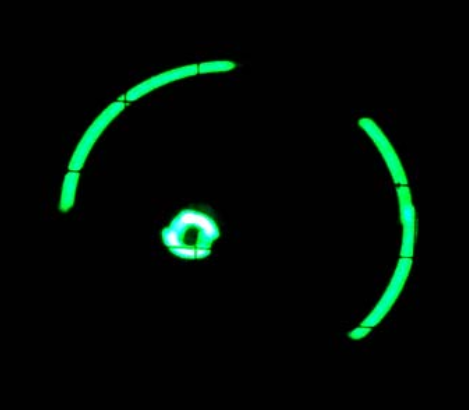
\includegraphics[width=0.5\linewidth]{figs/descripcion/juego.png}
    \caption{Captura de una partida del juego \cite{pong}}
    \label{ejemploJuego}
\end{figure}
\subsection{Descipción de cada etapa}
\subsubsection{Oscilador en cuadratura}
Esta etapa genera dos ondas sinusoidales, una desfasada 90° con respecto a la otra.
Dichas ondas sinusoidales son alimentadas a otras etapas del circuito para ser comparada con otras señales, o para ser procesadas. 
Esta es la etapa más esencial del circuito, debido a que estas ondas sinusoidales son las que se utilizan para dibujar arcos y círculos en el osciloscopio.
Esto es logrado por medio del modo XY del osciloscopio, en donde se toman los voltajes en dos de los canales de entrada del equipo y se grafican considerando que corresponden a coordenadas cartesianas. 
Un caso especial de esto es cuando se alimenta $\cos(\omega t)$ al canal asociado al eje X, y $\sin(\omega t)$ al canal asociado al eje Y. 
Esto genera un círculo en la pantalla del osciloscopio.
A partir de las transformaciones de estas señales analógicas y señales de control producidas por el resto de las etapas del circuito, se logra simular una pelota circular, paletas, y rebotes.

Se propone alterar el diseño original utilizando un oscilador de Bubba en vez de un oscilador en cuadratura, con el propósito de evaluar si un oscilador con esta topología tiene alguna ventaja con respecto al oscilador del diseño original. 
En la \figref{cuadraTopologies} se muestran ambas topologías de osciladores.

\begin{figure}[H]
    \centering
    \begin{minipage}{0.45\linewidth}
        \centering
        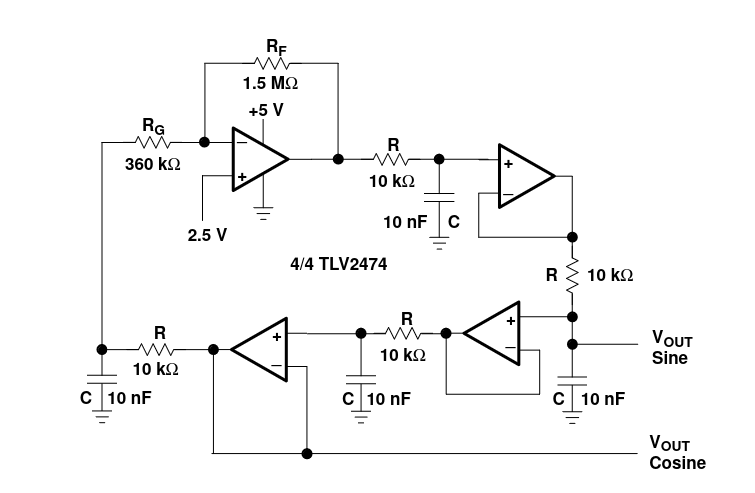
\includegraphics[width=1.1\linewidth]{figs/descripcion/bubba.png}
        \caption*{(a): Bubba \cite{opamps_everyone}}
    \end{minipage}
    \begin{minipage}{0.45\linewidth}
        \centering
        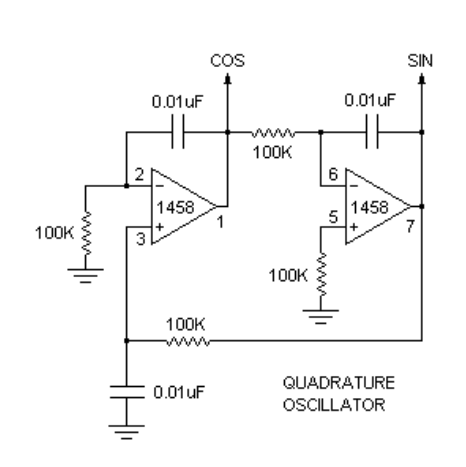
\includegraphics[width=0.8\linewidth]{figs/descripcion/oscilador_cuadratura.png}
        \caption*{(b): Original \cite{pong}}
    \end{minipage}
    \caption{Topologías de osciladores de cuadratura}
    \label{cuadraTopologies}
\end{figure}

\subsubsection{Circuito desfasador de 360°}
Esta etapa utiliza un potenciómetro de doble gang (Pot DG) con el cual se desfasa la señal sinusoidal de entrada en el rango de desfases $[0°,\,360°]$.
Las etapas siguientes aprovechan esta señal desfasada para ajustar la posición angular de la paleta, por lo que el jugador controla la posición de la paleta a través de dicho potenciómetro.
Hay dos circuitos como estos en el circuito, uno encargado de la paleta $A$ y otro de la paleta $B$.
En la \figref{desfasador}, se muestran dichos circuitos.

\begin{figure}[H]
    \centering
    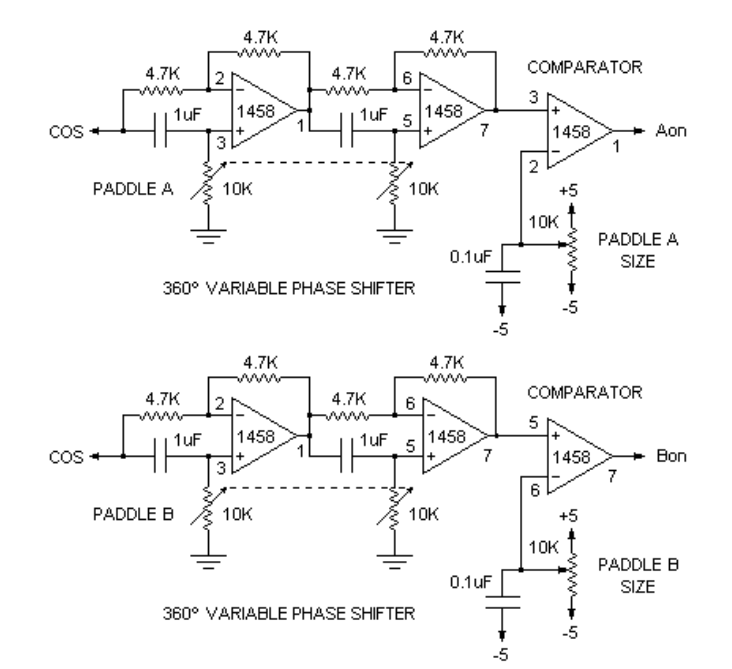
\includegraphics[width=0.5\linewidth]{figs/descripcion/desfasador}
    \caption{Circuitos desfasadores de 360° \cite{pong}}
    \label{desfasador}
\end{figure}

\subsubsection{Comparador ajustable}
Esta etapa genera una onda cuadrada en base a un nivel de tensión DC ajustado por medio de un potenciómetro. 
Esta etapa es conectada después de los circuitos desfasadores, como se muestra en la \figref{desfasador}.
Esto permite ajustar el tamaño de cada una de las paletas.
Se propone utilizar un potenciómetro de doble gang para ajustar el tamaño de las paletas, con el propósito de que el tamaño de estas sea simétrico. 
Estas ondas cuadradas son denominadas $A_{on}$ y $B_{on}$, una para cada paleta. 
Los tiempos que estas ondas están en alto indican los momentos en que se deben dibujar las paletas para lograr un tamaño en particular. 

\subsubsection{Comparador + flip flop}
Esta etapa genera una onda cuadrada con un ciclo de trabajo del 50\% aproximadamente, debido a que es producida a partir de la señal coseno proveniente del oscilador en cuadratura.
Gracias al uso de un flip flop en este circuito, como salidas de esta etapa se tienen las señales de reloj $CLK$ y $\overline{CLK}$, las cuales son utilizadas para generar distintas señales de control en el circuito.
Dicho circuito se muestra en la \figref{compFF}.

\textbf{Nota:} Para todas las etapas y señales del circuito que realicen algún procesamiento digital, se consideraron los niveles lógicos $V_H = \SI{5}{V}$ y $V_L = \SI{-5}{V}$.

\begin{figure}[H]
    \centering
    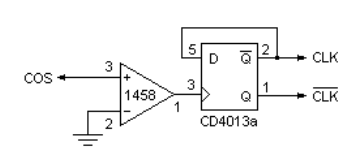
\includegraphics[width=0.5\linewidth]{figs/descripcion/comparadorFF.png}
    \caption{Circuito con comparador y flip-flop \cite{pong}}
    \label{compFF}
\end{figure}

\subsubsection{Control de dibujo y paleta}
Esta etapa realiza procesamiento digital únicamente.
La razón del porque el circuito ocupa señales de control se debe a que se quieren dibujar varios elementos en la pantalla del osciloscopio a la vez (paletas y pelota), y solo se tienen los canales de salida $ScopeX$ y $ScopeY$, los cuales se ocupan ambos cuando se quiere dibujar un elemento en particular en la pantalla. 
Se propone multiplexar todos los elementos que se desean dibujar en la pantalla, controlando los momentos de dibujado a través de distintas señales de control.
Esto es definido de la siguiente manera:
\begin{itemize}
    \item Si $CLK$ está en alto, se dibujan las paletas.
    \item Si $CLK$ está en bajo, se dibuja la pelota. 
\end{itemize}
Lo anterior se resume en la señal de control $T$, la cual es descrita a través de la función combinacional \eqref{T}.
\begin{equation}
    T = \overline{(A_{on} + B_{on})\cdot CLK}\label{T}
\end{equation}
La negación en esta función se debe a la polaridad de los switches analógicos utilizados para cambiar entre la señal de la paleta y la de la pelota, en la etapa ``Multiplexor analógico 2 a 1, sumador".
Dichos swithces analógicos son implementados utilizando el circuito integrado CD4066B, disponible para su compra en la tienda costarricense MicroJPM en el siguiente \href{https://www.microjpm.com/products/cd4066-ic-cmos-quad-bilateral-switch/}{enlace}.

Como se multiplexan las señales de la pelota y la paleta en la pantalla del osciloscopio, se debe realizar con cuidado la verificación del choque entre la pelota y la paleta. Esto debido a que ambas señales no están presentes en el circuito a la misma vez.
Por cuanto, es necesario una señal de control adicional, denominada $PL$, la cual es encargada de indicar el momento correcto en donde se puede dar un choque entre alguna de las paletas y la pelota, para que la señal $BOUNCE$ se ponga en alto en caso de que se de un choque. 
Dicha señal se muestra en la ecuación \eqref{PL}.
\begin{equation}
    PL = \overline{((A_{on}\cdot TURN + B_{on} \cdot\overline{TURN})\cdot\overline{CLK}}\label{PL}
\end{equation}
Note que esta ecuación es equivalente a \eqref{T}, con la excepción de que utiliza la señal $\overline{CLK}$, y combina las señales $TURN$ y $\overline{TURN}$ con las señales de las paletas correspondientes, con el propósito de verificar choques únicamente con la paleta del jugador que le toca el turno actual. 
El circuito que implementa esta etapa se muestra en la \figref{ccu}.

\begin{figure}[H]
    \centering
    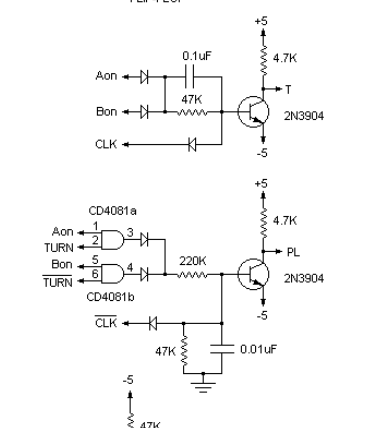
\includegraphics[width=0.5\linewidth]{figs/descripcion/ccu.png}
    \caption{Circuito para el control de dibujo y paleta \cite{pong}}
    \label{ccu}
\end{figure}

\subsubsection{Multiplexor analógico 2 a 1, sumador}
Esta etapa es la encargada de multiplexar las señales de la paleta y de la pelota. 
La paleta es dibujada a partir de las señales en cuadratura producidas por el oscilador, mientras que la pelota es dibujada reescalando dichas señales por medio de un divisor de tensión y sumandole un offset DC a estas señales en cuadratura.
Esto produce un círculo más pequeño que las pelotas que se puede desplazar por la pantalla del osciloscopio a partir del offset DC.
Dicho offset DC es manejado por la etapa ``Flip flop + circuito RC" con las señales $BallX$ y $BallY$.
La multiplexación es realizada por medio de un switch analógico, el cual conduce de acuerdo a lo dictado por la señal $T$ descrita por la ecuación \eqref{T}.
Este circuito se implementó para ambos canales del osciloscopio utilizado para dibujar el juego.
Dicho circuito se muestra en la \figref{mux}.

\begin{figure}[H]
    \centering
    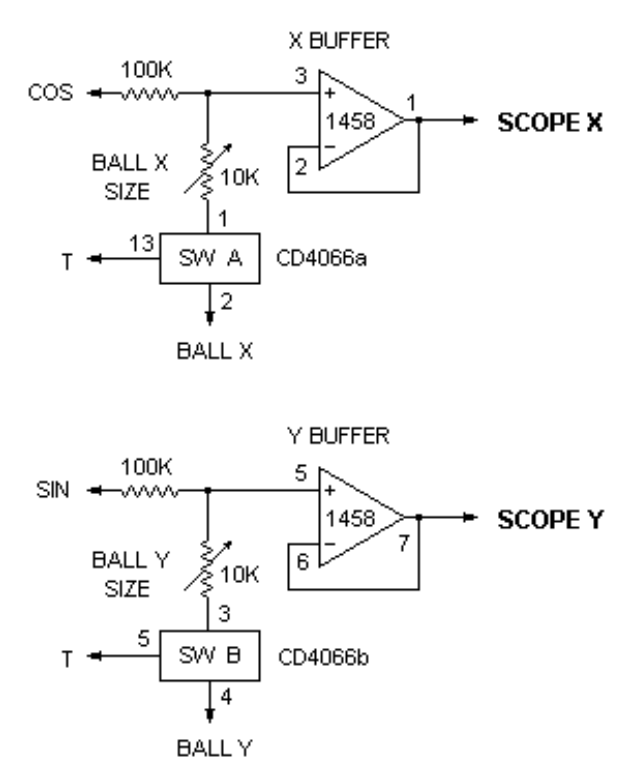
\includegraphics[width=0.5\linewidth]{figs/descripcion/multiplexor.png}
    \caption{Circuito multiplexor analógico 2 a 1, sumador \cite{pong}}
    \label{mux}
\end{figure}

Es importante resaltar que, como tal, este circuito no suma como un sumador convencional que utiliza amplificadores operacionales.
El circuito habilita y deshabilita un divisor de tensión, permitiendo escoger entre una señal en cuadratura (paletas), o una señal en cuadratura de menor amplitud y con un offset DC (pelota).

\subsubsection{Flip flop y circuito RC}
Esta etapa es la encargada de controlar la dinámica de la pelota. 
Cuando la pelota rebota, las señales $X_{rev}$ y $Y_{rev}$ conmutan, causando que cambie la salida del flip flop al que están conectadas estas señales, provocando que el capacitor en el circuito RC se cargue o descargue, produciendo las señales $BallX$ y $BallY$.
Esto simula el movimiento de la pelota, el cual es rápido al principio, y poco a poco se realentiza, hasta que la tensión del capacitor llega a estado estacionario. 
Es posible ajustar la velocidad de la pelota por medio de un potenciómetro de doble gang, el cual cambia la constante $\tau$ del circuito RC al rotar el potenciómetro, provocando una velocidad de carga o descarga distinta, acelerando o realentizando la pelota.
El circuito que implementa esta etapa se muestra en la \figref{ffRC}.

\begin{figure}[H]
    \centering
    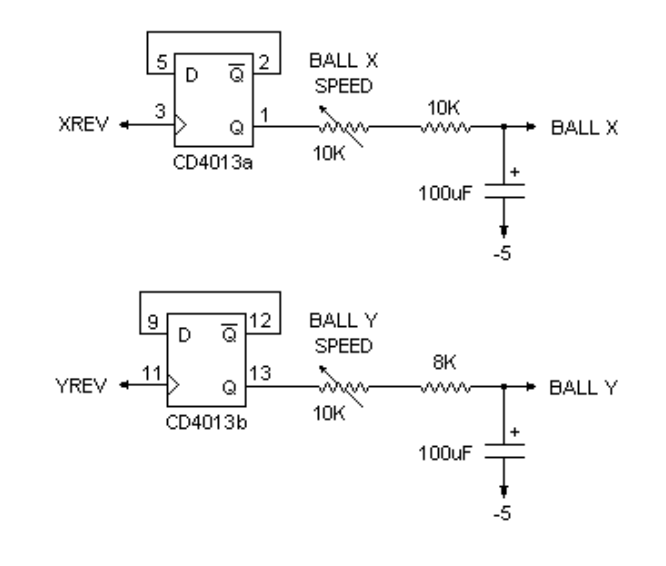
\includegraphics[width=0.5\linewidth]{figs/descripcion/ffRC.png}
    \caption{Circuito con flip flop y circuito RC \cite{pong}}
    \label{ffRC}
\end{figure}

\subsubsection{Comparadores de ventana}
Esta etapa es la encargada de determinar una colisión entre la paleta y la pelota.
Siempre y cuando las condiciones para que se de una colisión de acuerdo a la señal de control $PL$, si se da una colisión, los comparadores de ventana para el eje X y el eje Y se activan, provocando que la salida del circuito se ponga en alto, corrspondiente a la señal $BOUNCE$.
Se utiliza un switch analógico como pulldown para la señal $BOUNCE$ en caso de que $PL$ esté en alto (es decir, no es posible que se de un rebote en estas condiciones).
El circuito que implementa esta etapa se muestra en la \figref{comparadores}.

\begin{figure}[H]
    \centering
    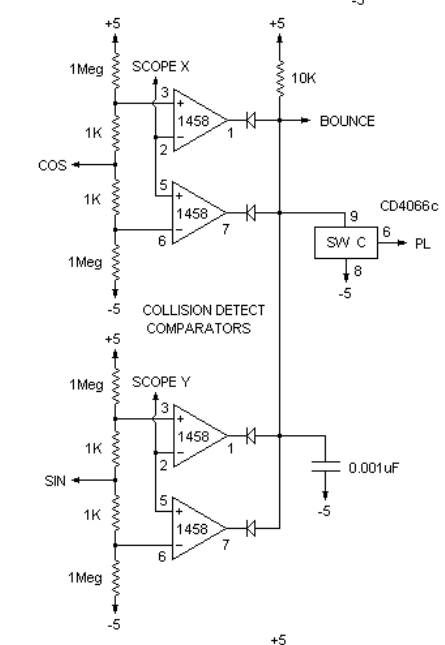
\includegraphics[width=0.5\linewidth]{figs/descripcion/comparadores}
    \caption{Circuitos comparadores de ventana \cite{pong}}
    \label{comparadores}
\end{figure}

\subsubsection{Comparadores de ventana (límites horizontales/verticales)}
Esta etapa es encargada de determinar si la pelota ha llegado a los límites de la pantalla del juego.
Las señales de salida $XR$ y $YR$ son utilizadas para ejecutar un rebote, en caso de que $BOUNCE$ se ponga en alto también cuando $XR$ y $YR$ lo hagan. 
El circuito que implementa esta etapa se muestra en la \figref{limites}.

\begin{figure}[H]
    \centering
    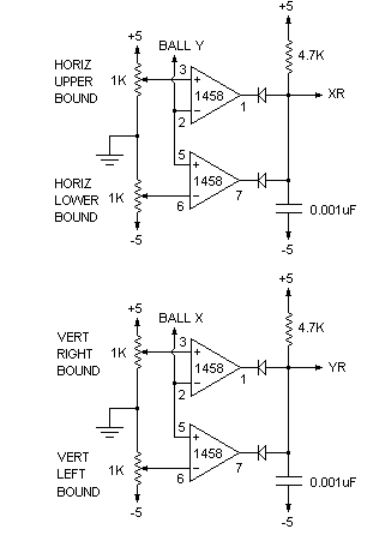
\includegraphics[width=0.5\linewidth]{figs/descripcion/hv.png}
    \caption{Circuitos comparadores de ventana para los límites horizontales y verticales de la pantalla del juego \cite{pong}}
    \label{limites}
\end{figure}

\subsubsection{Control de dirección de la pelota}
Esta etapa se encarga de controlar a que próxima dirección se moverá la pelota.
Cuando $XR$ y $BOUNCE$, o $YR$ y $BOUNCE$ se ponen en alto, las señales $X_{rev}$ o $Y_{rev}$ conmutan, provocando que la pelota rebote en alguna dirección debido a las etapas ``flip flop + circuito RC" y también ``Mux analógico 2 a 1, sumador". 
Adicionalmente, este circuito proporciona un botón de reinicio, que al ser presionado, coloca la pelota en el centro de la pantalla.
Esto es útil en caso de que la pelota se haya desplazado a alguno de los límites de la pantalla y no sea posible recuperarla por medio de las paletas.
El circuito que implementa esta etapa se muestra en la \figref{controlPelota}.

\begin{figure}[H]
    \centering
    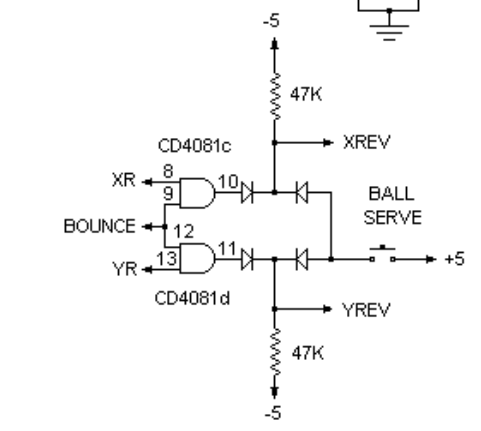
\includegraphics[width=0.5\linewidth]{figs/descripcion/controlPelota.png}
    \caption{Circuito para el control de dirección de la pelota \cite{pong}}
    \label{controlPelota}
\end{figure}

\subsubsection{Control de turnos y LEDs indicadores}
Esta etapa se encarga de controlar las señales $TURN$ y $\overline{TURN}$, así como dos LEDs indicadores que le indican a los jugadores de quien es el turno actual. 
El circuito consiste simplemente de un flip flop, y una rama con LEDs y resistencia para regular la corriente. 
Cuando haya un flanco positivo en $BOUNCE$, las salidas del flip flop conmutan, provocando que un LED se apague y otro se prenda, permitiendo identificar de cual jugador es el turno actual.
El circuito que implementa esta etapa se muestra en la \figref{turnos}.

\begin{figure}[H]
    \centering
    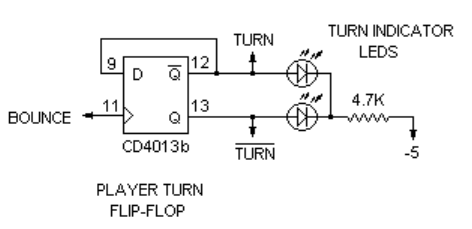
\includegraphics[width=0.5\linewidth]{figs/descripcion/turnos.png}
    \caption{Circuito para el control de turnos y LEDs indicadores \cite{pong}}
    \label{turnos}
\end{figure}

\subsubsection{Efectos de sonido}
Este circuito genera un zumbido cada vez la bola rebota en alguan de las paletas.
Esto es logrado por medio de un buzzer.
El circuito que realiza esta función se muestra en la \figref{sonido}.

\begin{figure}[H]
    \centering
    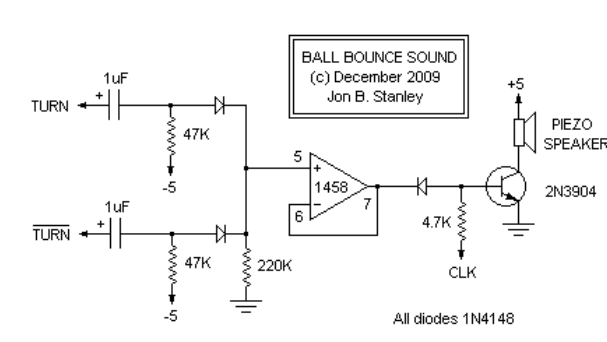
\includegraphics[width=0.5\linewidth]{figs/descripcion/sonido.png}
    \caption{Circuito para efectos de sonido \cite{pong}}
    \label{sonido}
\end{figure}

\subsection{Diagrama de bloques}
En la \figref{ohmpong} se muestra un diagrama de bloques que incluye cada una de las etapas mencionadas anteriormente.

\begin{figure}[H]
    \centering
    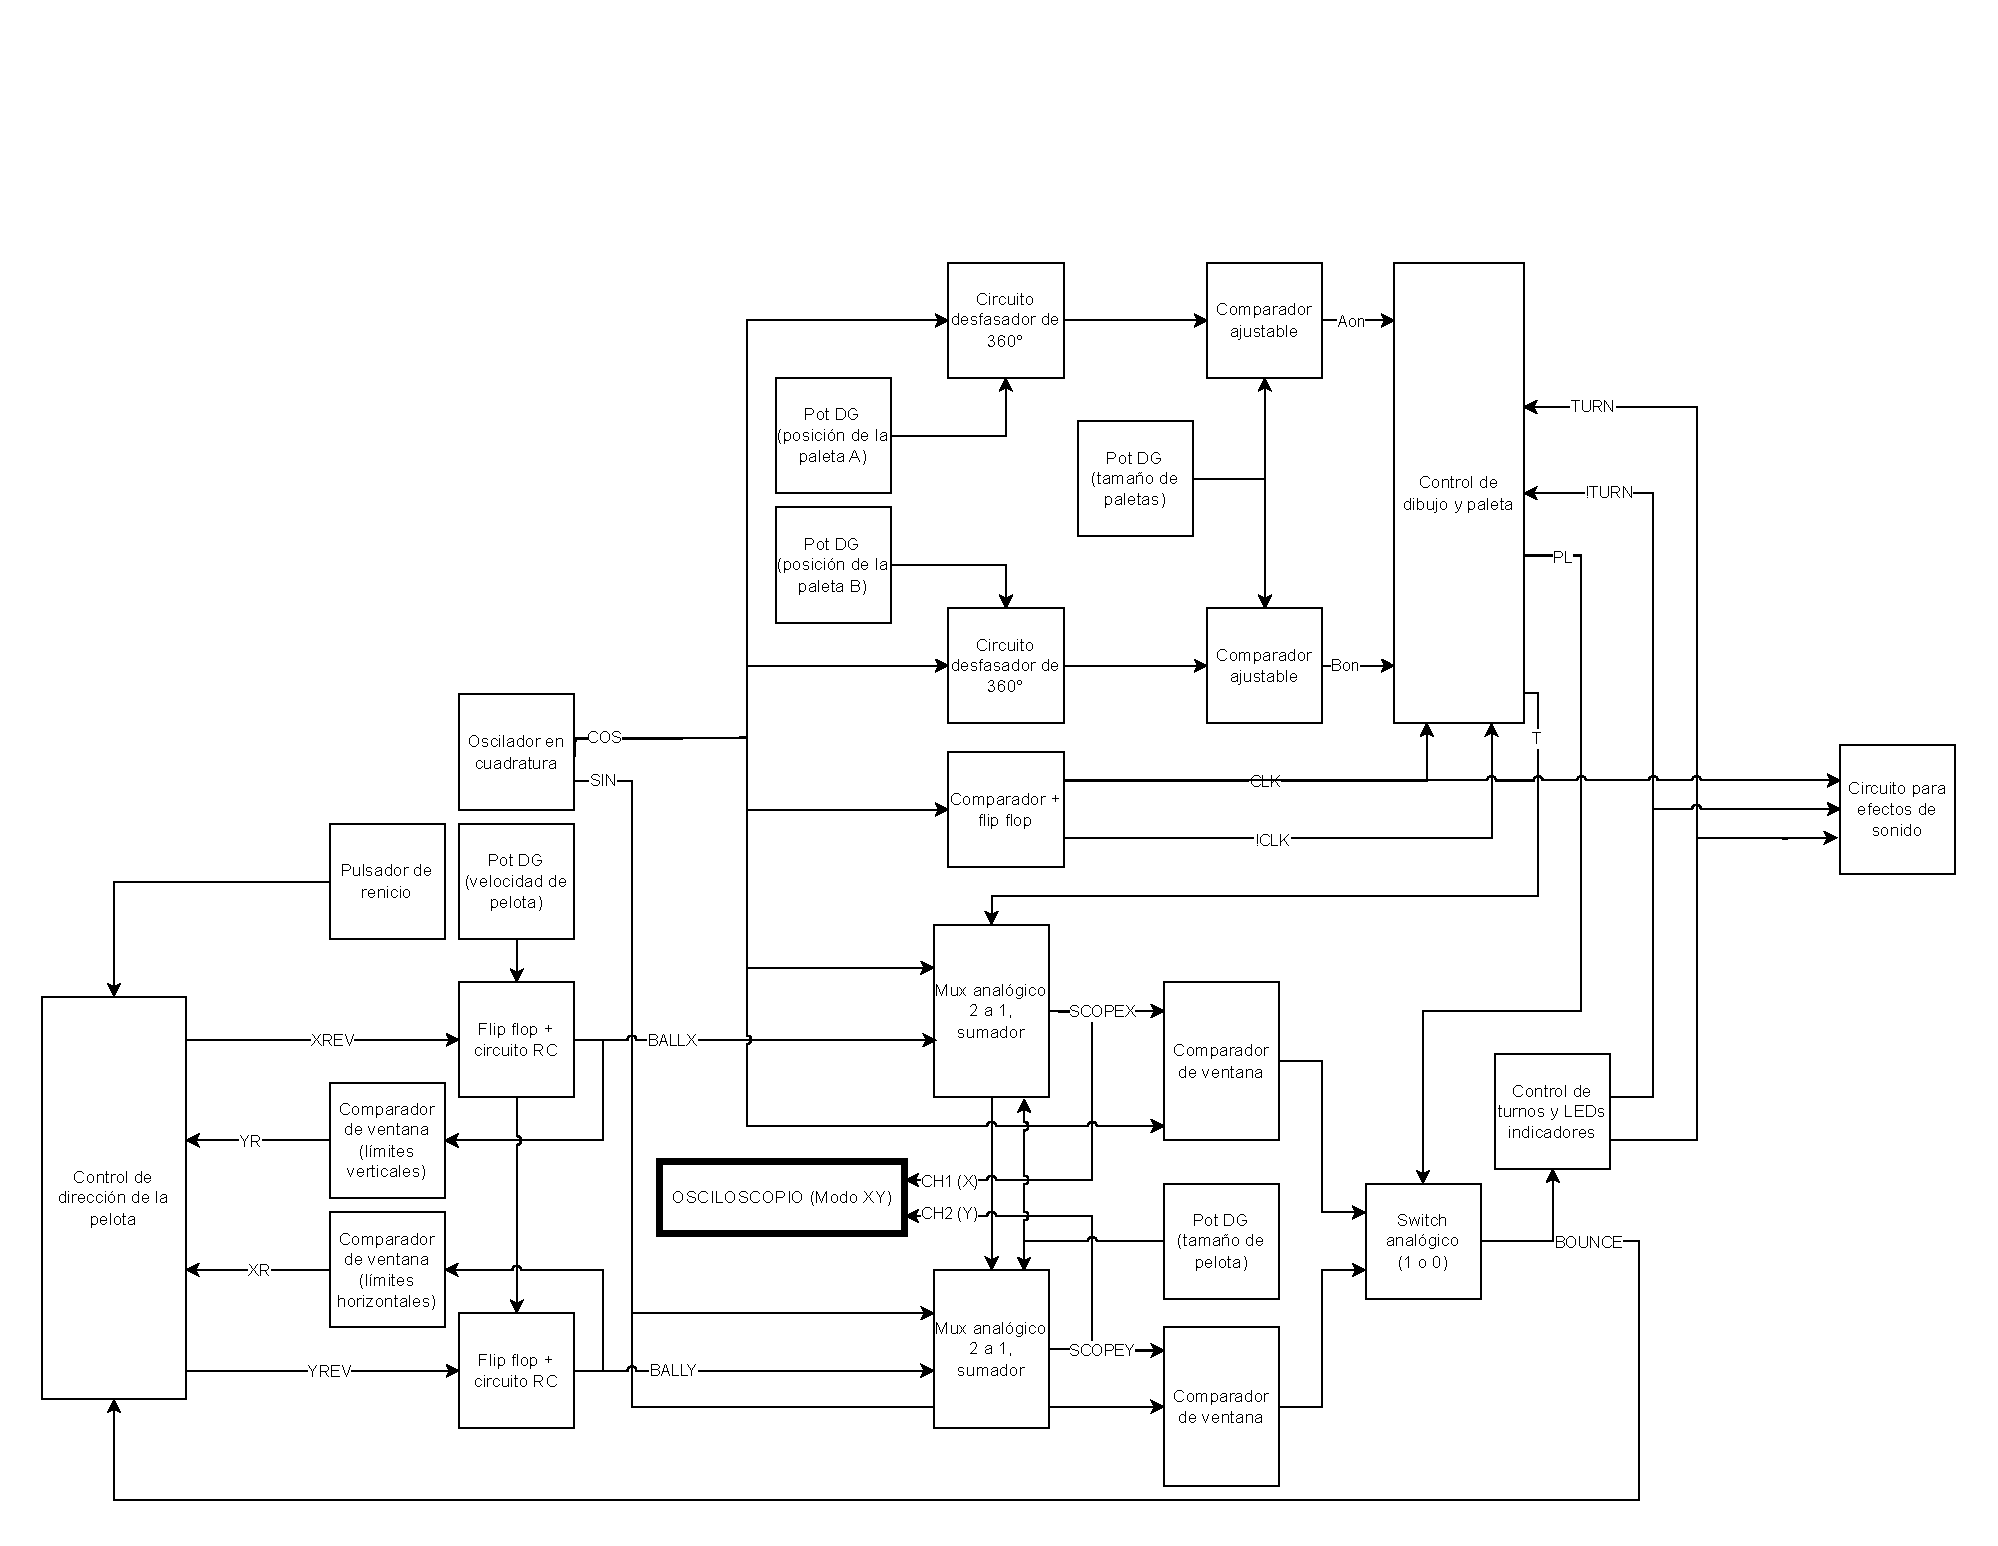
\includegraphics[width=\linewidth]{figs/db/PongO.pdf}
    \caption{Diagrama de bloques de $\Omega$--Pong}
    \label{ohmpong}
\end{figure}